\chapter{(E) Processi stocastici} \label{cap:bimodal}

\section{(E-1) Sviluppo del processo lognormale a variabile stocastica binaria}

La determinazione del prezzo di un prodotto derivato è indissolubilmente legata all'andamento teorico del valore del sottostante. Data questa premessa, un equo \textit{pricing} delle opzioni non può prescindere da una previsione il più accurata possibile dell'andamento di tale valore. Nella Sezione \ref{sec:introduction_econophysic_option_pricing} è stato indicato lo schema del moto browniano geometrico come particolarmente valido per questo tipo di modellizzazione. Il processo lognormale con cui evolve il prezzo del sottostante è un processo di tipo markoviano descritto, come si è visto, dall'equazione a schema esatto \eqref{eq:exactprice}, dove $w$ rappresenta una variabile aleatoria a media nulla e varianza unitaria.

Nell'ottica di riprodurre con la maggiore fedeltà possibile un'ipotetica evoluzione dei prezzi del sottostante, il termine $w$ è stato estratto da una distribuzione gaussiana. Successivamente, a titolo di confronto, abbiamo implementato nella classe \codeword{RNG} e le sue derivate una nuova funzione \codeword{GetBimodal()} che genera una variabile stocastica dicotomica
\begin{equation}
    z = \begin{cases}
    +1, & \text{con probabilità} \,\, \frac{1}{2};\\
    -1, & \text{con probabilità} \,\, \frac{1}{2}.
  \end{cases}
    \label{eq:binary_variable}
\end{equation}
Abbiamo quindi applicato iterativamente il processo lognormale 
\begin{equation}
    S\left(t_{i+1}\right) = S(t_i) \exp{\left[\left(r - \frac{\sigma^2}{2}\right) \Delta t + \sigma \sqrt{\Delta t} z\right]}
    \label{eq:bimodal_price}
\end{equation}
con questa nuova variabile per valutare l'effetto che essa induce sulla stima del prezzo dell'opzione se raffrontata ai risultati conseguiti con una variabile gaussiana $w$.

Nel caso dicotomico, per ogni intervallo temporale $\Delta t$ il valore di $S(t_{i + 1})$ è vincolato a due sole possibilità rispetto a $S(t_i)$, ovvero quella di un movimento al rialzo, se $z = 1$, o al ribasso, se $z = -1$. A ogni passo della simulazione il prezzo $S(t)$ può quindi assumere due soli valori dipendenti dal risultato del passo precedente, dalla volatilità $\sigma$, dal tasso di interesse privo di rischio $r$ e dalla scelta dell'intervallo stesso $\Delta t$, in contrapposizione allo spettro continuo di valori del processo lognormale standard.

\section{(E-2) Convergenza del processo binario al processo lognormale gaussiano}

Sia che si scelga di utilizzare una variabile $w$ a distribuzione gaussiana, sia che il termine aleatorio sia di tipo bimodale $z$, la funzione \codeword{ExactLogNormalStep(...)}, che prende in ingresso la variabile stocastica e restituisce il prezzo del sottostante alla data di rilevazione considerata, è la medesima, in quanto l'equazione \eqref{eq:exactprice} si applica identicamente all'uno e all'altro caso. 

Abbiamo eseguito una serie di coppie di simulazioni identiche a eccezione del tipo di parametro pseudocasuale passato alle funzioni del processo lognormale. In questo modo è stato possibile confrontare i risultati relativi a entrambe le scelte del termine aleatorio per verificarne la convergenza.

In particolare, le simulazioni prese in esame per la comparazione stimano il prezzo di opzioni del tipo \textit{plain vanilla call} a partire dai seguenti dati di \textit{input}:
\begin{itemize}
    \item numero di simulazioni $N={10}^7$;
    \item numero di intervalli temporali $m$ variabile tra $1$ e $350$.
\end{itemize}
In Figura \ref{fig:bimodal} sono riportati i risultati ottenuti per mezzo del processo lognormale esatto nel caso di impiego di una variabile gaussiana (in grigio, tratteggiato) oppure di una bimodale (in magenta).

\begin{figure}[t]
    \centering
    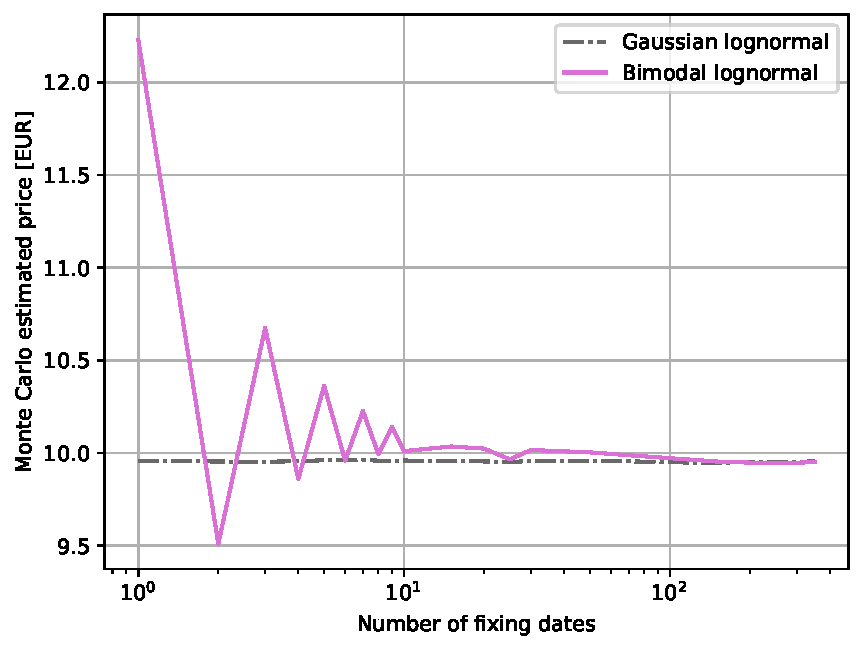
\includegraphics[scale=0.5]{graphs/OptionPriceBimodal_PriceVsM.pdf}
    \caption[Confronto tra il prezzo stimato dell'opzione \textit{performance corridor} sfruttando variabili  bimodali e gaussiane di media nulla e varianza unitaria.]{Prezzo stimato dell'opzione \textit{performance corridor} tramite lo schema lognormale esatto sfruttando variabili pseudocasuali bimodali (in \textit{magenta}) e gaussiane di media nulla e varianza unitaria (in \textit{grigio, tratteggiato}).}
    \label{fig:bimodal}
\end{figure}

L'evoluzione delle due curve incontra le nostre aspettative: si nota infatti come, dopo un'iniziale fase discordante, i due sviluppi tendano a sovrapporsi e in particolare sia l'andamento della curva a variabile bimodale a stabilizzarsi fino a convergere sui risultati di quella a variabile gaussiana.
%La spiegazione risiede nella natura \textit{markoviana} del processo di calcolo: lo schema lognormale si basa su una successione ricorsiva che estrapola il prezzo al tempo $t_i$ a partire da quello alla data precedente $t_{i-1}$. Di conseguenza, nel caso non ci siano <<tappe temporali intermedie>>, i prezzi al \textit{tempo di maturità} sono l'esito di un'unica operazione in positivo o negativo. I risultati ottenuti dal singolo \textit{thread} si raggruppano dunque in due classi di prezzi. Incrementando il numero di passaggi intermedi aumenta il ventaglio di prezzi ottenibili dalla singola simulazione. Per una densità di date di rilevazione sufficientemente elevata i due processi danno risultati confrontabili, sebbene l'impiego di una variabile dicotomica non permetta di parlare di tendenza asintotica; infatti, al crescere di $m$ il prezzo finale del metodo binario non si avvicina indefinitamente <<dall'alto>> o <<dal basso>> al valore gaussiano.
Una spiegazione matematica di questo comportamento è fornita dal \textit{teorema del limite centrale}, secondo il quale la somma di $N$ variabili aleatorie $x_n$ indipendenti e identicamente distribuite tende, per $N \rightarrow \infty$, a seguire una distribuzione normale di media $N\braket{x_n}$ e varianza $N\text{Var}[x_n]$.

Considerando ora l'equazione che descrive l'andamento del prezzo del sottostante in funzione di $\Delta t$ e del numero $m$ di sottointervalli temporali di rilevazione
\begin{equation}
    S(m \Delta t) = S(0) \exp{\left[m \left(r - \frac{\sigma^2}{2}\right) \Delta t + \sigma \sqrt{\Delta t} \displaystyle\sum_{i=1}^m z_i\right]},
    \label{eq:price(n)}
\end{equation}
si può pensare di definire una nuova variabile aleatoria
\begin{equation}
   Y(m) := \displaystyle\sum_{i=1}^m z_i.
\end{equation}

Le variabili ${z_i}$, siano esse bimodali o gaussiane, sono  pseudocasuali, indipendenti ed estratte secondo la medesima distribuzione: essendo soddisfatte le ipotesi del teorema del limite centrale, $Y(m)$ è quindi a sua volta una variabile che segue una distribuzione normale con media
\begin{equation}
    \braket{Y(m)} = m\braket{z_i} = 0,
\end{equation}
e varianza
\begin{equation}
    \text{Var}[Y(m)] = m\text{Var}[z_i] = m.
\end{equation}

La ragione della convergenza risiede dunque nel fatto che le variabili gaussiane e bimodali sono estratte con medesima media nulla e varianza unitaria, il che, in virtù del teorema del limite centrale, porta $Y(m)$ a coincidere nei due casi per $m\gtrsim 100$; al di sotto di tale limite il teorema non è più valido e la natura dicotomica della variabile $z$ induce la dispersione osservabile rispetto al processo lognormale standard. L'andamento riscontrato nelle simulazioni ha quindi una comprova teorica.
